% !TeX root = RJwrapper.tex

\newcommand{\rev}[1]{{\color{red} #1}}


\title{Spatio-Temporal Interpolation using \pkg{gstat}}
% \VignetteIndexEntry{Spatio-Temporal Geostatistics using gstat}

\author{by Benedikt Gr{\"a}ler, Edzer Pebesma and Gerard Heuvelink}

\graphicspath{{figures/}}

\maketitle

\abstract{
We present new spatio-temporal geostatistical modelling and interpolation capabilities of the R package \pkg{gstat}. Various spatio-temporal covariance models have been implemented, such as the separable, product-sum, metric and sum-metric models. In a real-world application we compare spatio-temporal interpolations using these models with a purely spatial kriging approach. The target variable of the application is the daily mean $\rm{PM}_{10}$ concentration measured at rural air quality monitoring stations across Germany in 2005. R code for variogram fitting and interpolation is presented in this paper to illustrate the workflow of spatio-temporal interpolation using \pkg{gstat}. We conclude that the system works properly and that the extension of \pkg{gstat} facilitates and eases spatio-temporal geostatistical modelling and prediction for R users.
}

%% main text
\section{Introduction}\label{sec:intro}
The collection and processing of spatio-temporal data is rapidly increasing due to technological advances and the societal need for analysis of variables that vary in space and time, such as weather and air quality variables, and crop yields. Analysis of spatial and temporal correlations is useful in itself to get insight into the character and causes of variability, but they are also important to predict values at points from neighbouring observations. Spatio-temporal interpolation can potentially provide more accurate predictions than spatial interpolation because observations taken at other times can be included. In addition, spatio-temporal interpolation allows predictions to be made at single locations or entire fields in between and beyond observation times. However, adding the temporal domain implies that variability in space and time must be modelled, which is more complicated than modelling purely spatial or purely temporal variability. The spatial, temporal and spatio-temporal dependence structures, for instance represented as variograms, do not necessarily coincide with each other in terms of their parameters nor in terms of their family. In the simplest case, a spatio-temporal anisotropy parameter might be enough to deal with the different dependence structures, but this poses strong assumptions on the process. 

Interpolation of spatial random fields is a common task in geostatistics. Simple approaches like inverse distance weighted predictions or the well known kriging procedures have routinely been applied for many years. Nowadays, modern sensors allow to monitor different variables at an increasing temporal resolution producing rich spatio-temporal data sets.
This calls as well for theory and methods to deal with these data sets to gain a better understanding of the observed spatio-temporal processes. While the theoretical aspects of spatio-temporal geostatistics show good progress \citep{Cressie2011}, implementations lack behind. This hinders a wide application of spatio-temporal modelling, as typically extensive scripting and thorough understanding is necessary to build spatio-temporal models. Handling of spatio-temporal data in R is provided by the \CRANpkg{spacetime} package \citep{Pebesma2012}. In this paper, we present an extension of the \CRANpkg{gstat} package \citep{Pebesma2004} (version 1.1-3) that reuses the \pkg{spacetime} classes for the estimation of spatio-temporal covariance/variogram models and to perform spatio-temporal interpolation. Our implementation handles various types of spatio-temporal covariance structures and facilitates spatio-temporal interpolation. The notation of functions in \pkg{gstat} are extended in a way closely following the purely spatial design. This allows a researcher acquainted with \pkg{gstat} to readily use spatio-temporal tools. The use of the newly implemented functions is presented and illustrated by mapping spatio-temporal air-quality data. Another package that offers extensive spatio-temporal geostatistical functionality is \CRANpkg{RandomFields} \citep{Schlather2014}; further packages are mentioned in the SpatioTemporal CRAN task view\footnote{\url{http://cran.r-project.org/web/views/SpatioTemporal.html}}.

The paper is organised as follows. The next section introduces the general interpolation routine and describes the different spatio-temporal covariance models, followed by a section introducing the German rural background data set for 2005 and performing the parameter estimation (i.e. covariance model fitting). Cross-validation results are presented and discussed in the section thereafter. Conclusions are drawn in the closing section. R scripts reproducing this study are available from within the \pkg{gstat} package as demos. \code{stkrige} re-estimates the variogram models, \code{stkrige-prediction} re-executes the prediction for a time series and a couple of stations, and \code{stkrige-crossvalidation} re-runs the entire leave-one-out cross-validation (note that the latter takes a few hours).

\section{Spatio-temporal dependence modelling and kriging}\label{sec:theory}

In the following, we will assume a Gaussian spatio-temporal random field $Z$ defined over a spatial domain $\mathcal{S}$ and temporal domain $\mathcal{T}$. Typically, a sample $\mathbf{z} = \big(z(s_1,t_1),\dots,z(s_n,t_n)\big)$ has been observed at a set of distinct spatio-temporal locations $(s_1, t_1), \dots, (s_n,t_n) \in \mathcal{S}\times \mathcal{T} \subseteq \mathbb{R}^2 \times \mathbb{R}$ that may include repeated measurements at the same location or simultaneous measurements at multiple spatial locations. Often, one is interested in modelling $Z$ from the sample $\mathbf{z}$ in order to predict at unobserved locations in space and time or simulate from the conditional distribution.

Across our domain of interest $\mathcal{S} \times \mathcal{T}$, we assume the random field $Z$ to be stationary and spatially isotropic. Hence, the field can be characterised through a mean $\mu$ and a covariance function $C_{\rm st}$ where the spatio-temporal covariance only depends on the separating distances across space $h \in \mathbb{R}_{\geq 0}$ and time $u \in \mathbb{R}_{\geq 0}$. Note that extensions beyond this set-up can easily be derived as has been done for the pure spatial case using for instance universal kriging to overcome the stationarity of the mean. The general spatio-temporal covariance function is given by
$C_{\rm st}(h,u) = {\rm Cov}\big(Z(s,t), Z(\tilde{s},\tilde{t})\big)$ 
for a separating spatial distance $h$ and temporal distance $u$ and any pair of points $(s,t), (\tilde{s},\tilde{t}) \in \mathcal{S}\times\mathcal{T}$ with $||s-\tilde{s}||=h$ and $|t-\tilde{t}|=u$. In general, this covariance function is hard to estimate but a couple of models using simplifying assumptions will be presented in the following together with their spatio-temporal variograms $\gamma_{\rm st}(h,u) = C_{\rm st}(0,0)-C_{\rm st}(h,u)$ and encoding in \pkg{gstat}. Given a valid covariance function, the covariance matrices used in the linear predictor are easily obtained and the same algebraic operations as in the well known spatial case yield predictions of the desired random field \citep{Cressie2011}. A major difference is, however, the computational complexity of the matrix inversion. Typically, observations are made at a rather high temporal frequency leading to a number of spatio-temporal locations that is too large for global kriging. Hence, interpolation based on a selected neighbourhood of a subset of all data points becomes beneficial. Additionally, this relaxes the assumption of stationarity, as smooth variations in the mean value across the domain can be respected. The related class of dynamic models also addresses the computational complexity resulting in a temporal Markov structure. Implementations can be found in \CRANpkg{spTimer} by \citet{bakar2015}, \CRANpkg{spBayes} by \citet{finley2015}, \CRANpkg{spate} by \citet{sigrist2015} or \pkg{INLA} by \citet{lindgren2015}.

\subsection{Covariance models}

The covariance models implemented in \pkg{gstat} and presented in this paper are introduced in the following. Besides further extensions we focus on the basic classes of the \emph{separable}, \emph{product-sum}, \emph{metric} and \emph{sum-metric} spatio-temporal covariance functions. The building blocks (in the following denoted as \code{spatialVgm}, \code{temporalVgm} or \code{jointVgm}) of the spatio-temporal covariance functions are any of the purely spatial variogram models already available in \pkg{gstat}. Each one of the building blocks is created by a call of the function \code{gstat::vgm()}. Remaining arguments such as \code{sill} (the joint sill), \code{nug} (the joint nugget component) or \code{stAni} (the spatio-temporal anisotropy used in the \code{jointVgm}) are scalars and refer to parameters of the entire spatio-temporal covariance function:

\begin{enumerate}[a)]
\item The \dfn{separable covariance model} assumes that the spatio-temporal covariance function can be represented as the product of a spatial and temporal term:
$$C_{\rm sep}(h,u)=C_{\rm s}(h)C_t(u)$$ 
Its variogram is given by (see Appendix for details):
$$\gamma_{\rm sep}(h,u) = {\rm sill} \cdot \big( \bar{\gamma}_s(h)+\bar{\gamma}_t(u)-\bar{\gamma}_s(h)\bar{\gamma}_t(u) \big)$$

where $\bar{\gamma}_s$ and $\bar{\gamma}_t$ are standardised spatial and temporal variograms with separate nugget effects and (joint) sill of 1. The overall sill parameter is denoted by "sill". 

The R package \pkg{gstat} encodes this model as:

\code{vgmST("separable", space=spatialVgm, time=temporalVgm, sill=sill)}

The separable model has a strong computational advantage in the setting where each spatial location has an observation at each temporal instance (a \code{"STFDF"} without \samp{NA}s, \cite{Pebesma2012}). In these cases, the covariance matrix (and its inverse) can be composed using the Kronecker-product of the purely spatial and purely temporal covariance matrices (respectively their inverse).

\item 
The above model extends to the \dfn{product-sum covariance model} that we give here in a slightly different notation as \citet{DeCesare2001} and \citet{DeIaco2001} by 
$$C_{\rm ps}(h,u)=k C_{\rm s}(h)C_{\rm t}(u) + C_{\rm s}(h) + C_{\rm t}(u)$$

with $k > 0$.

The corresponding variogram can be written as
$$\gamma_{\rm ps}(h,u) = (k \cdot {\rm sill}_{\rm t} + 1) \gamma_{\rm s}(h) + (k \cdot {\rm sill}_{\rm s} + 1) \gamma_{\rm t}(u) - k \gamma_{\rm s}(h) \gamma_{\rm t}(u)$$

where ${\gamma}_{\rm s}$ and $\gamma_{\rm t}$ are spatial and temporal variograms (see Appendix for details). The parameter $k$ needs to be positive and the following identity defines the overall sill (${\rm sill}_{\rm st}$) of the model in terms of the model's spatial and temporal sills:
$${\rm sill}_{\rm st} = k \cdot {\rm sill}_{\rm s} \cdot {\rm sill}_{\rm t} + {\rm sill}_{\rm s} + {\rm sill}_{\rm t}.$$
The above equation can also be used to estimate $k$ based on the three sill values. An alternative formulation of the product-sum variogram can be found in \citet{DeIaco2001}.

The \pkg{gstat} definition of this model reads:

\begin{example*}
vgmST("productSum", space = spatialVgm, time = temporalVgm, k = k)
\end{example*}

\item 
Assuming identical spatial and temporal covariance functions except for spatio-temporal anisotropy, allows to use a spatio-temporal \dfn{metric covariance model} where, after matching space and time by an anisotropy correction $\kappa$ (\code{stAni}), the spatial, temporal and spatio-temporal distances are treated equally resulting in a single covariance model $C_{\rm joint}$: 
$$C_{\rm m}(h,u)=C_{\rm joint}\big(\sqrt{h^2+(\kappa\cdot u)^2}\big)$$

The variogram evaluates to
$$ \gamma_{\rm m} (h,u) = \gamma_{\rm joint}(\sqrt{h^2+(\kappa\cdot u)^2}) $$
where $\gamma_{\rm joint}$ (\code{jointVgm}) is any known variogram that may include a nugget effect. The following line generates the model in \pkg{gstat}:

\begin{example*}
vgmST("metric", joint = jointVgm, stAni = stAni)
\end{example*}

The spatio-temporal anisotropy parameter $\kappa$ (\code{stAni}) is given as spatial unit per temporal unit. In many cases, this will be in m/second, as these are the base units in our implementation. All temporal distances are hence internally re-scaled to an equivalent spatial distance using \code{stAni} and treated as metric 3D-space.

\item
A combination of spatial, temporal and a metric model including an anisotropy parameter $\kappa$ is found in \citet{Bilonick1988} and revisited by \citet{Snepvangers2003} as the \dfn{sum-metric covariance model}: 
$$C_{\rm sm}(h,u)=C_{\rm s}(h)+C_{\rm t}(u)+C_{\rm joint}\big(\sqrt{h^2+(\kappa\cdot u)^2}\big)$$ 
This model allows for spatial, temporal and joint nugget effects. Thus, the variogram is given by
$$ \gamma_{\rm sm}(h,u)= \gamma_{\rm  s}(h) + \gamma_{\rm t}(u) + \gamma_{\rm joint}(\sqrt{h^2+(\kappa\cdot u)^2})$$
where $\gamma_{\rm s}$, $\gamma_{\rm t}$ and $\gamma_{\rm joint}$ are spatial, temporal and joint variograms with separate nugget-effects. This model can be defined in \pkg{gstat} through:

\begin{example*}
vgmST("sumMetric", space = spatialVgm, time = temporalVgm, joint = jointVgm,
      stAni = stAni)
\end{example*}

\item
A simplified version of the above model is to restrict the spatial, temporal and joint variograms to nugget free models. Additionally, a single spatio-temporal nugget is introduced and the variogram takes the representation:
$$\gamma_{\rm ssm}(h,u) = {\rm nug}\cdot {\bf1}_{h>0 \vee u>0} + \gamma_{\rm s}(h) + \gamma_{\rm t}(u) + \gamma_{\rm joint}(\sqrt{h^2+(\kappa\cdot u)^2})$$

The \dfn{simple sum-metric covariance model} can be obtained by:

\begin{example*}
vgmST("simpleSumMetric", space = spatialVgm, time = temporalVgm,
      joint = jointVgm, nugget = nug, stAni = stAni)
\end{example*}
\end{enumerate}

\noindent Note that the above mentioned spatial, temporal and joint components of the spatio-temporal covariance and variogram models need not necessarily exhibit the same structure. Taking for instance the product-sum and sum-metric models that both contain single temporal and spatial variogram models: the best fits of the respective spatio-temporal models might suggest different variogram families and parameters for the pure spatial and temporal ones. This is due to the target of finding the best overall variogram surface resulting in (potentially) different marginal models.

\subsection{Parameter estimation}

Fitting routines for the above variogram models are implemented in \pkg{gstat} through the function \code{fit.StVariogram()}, which calls \code{optim()} from the R core package \pkg{stats} \citep{RCoreTeam2016}. Additional parameters to improve the numerical optimisation can be provided to \code{fit.StVariogram()} and will be passed on to \code{optim()} (using R's three-dots mechanism). As some of the parameters are limited to certain ranges (nuggets need to be non-negative, ranges must be positive), it is advised to use an optimisation routine that allows to impose limits on the search space (i.e. \code{L-BFGS-B}) and provide sensible limits via \code{lower} and \code{upper}. By default, the method \code{L-BFGS-B} is called and the smallest lower and largest upper bounds supported by the model are given. The estimation of the spatio-temporal variogram models relies on a sample variogram empirically derived from the data. In contrast to the spatial variogram line, the spatio-temporal variogram is represented by a surface for lag classes composed of a spatial and temporal separation distance. Different from the spatial case, a spatio-temporal sample variogram contains lag-classes of zero spatial separation describing pure temporal dependencies. Without duplicate observations, no estimates can be made for the lag-class with both zero spatial and zero temporal separation. The sample variogram is calculated through the function \code{variogram()} that dispatches the call for spatio-temporal data objects (of class \code{"STFDF"}, \code{"STSDF"}, or \code{"STIDF"}) from \pkg{spacetime}. For a visual judgement of the fit between sample and fitted variograms the \code{plot()} function can be called to show the variogram surfaces next to each other as coloured level plots. Alternatively, a wireframe plot is obtained by setting the parameter  \code{wireframe = TRUE} (Figure~\ref{fig:allVgmsWireframe}). A further option is to plot the differences between the sample and model variogram surfaces by setting \code{diff = TRUE}, see Figure~\ref{fig:allVgmsDiffWireframe}. Additionally to visual comparison, \code{fit.StVariogram()} provides the output of \code{optim} as attribute \code{optim.out} of the returned S3-class \code{"StVariogram"}. This attribute includes valuable information to diagnose the success of the \code{optim} routine. It contains for instance the convergence code (\code{\$convergence}) or message (\code{\$message}) and  the optimised value (\code{\$value}), which is the mean of the (weighted) squared deviations between sample and fitted variogram surface. Furthermore, it is advised to check the estimated parameters against the parameter boundaries and starting values. Additionally, starting values might also influence the success and result of the optimisation, as local optima may occur due to the interdependence of the parameters. Alternatively, the user might want to start a grid search in order to better asses the sensitivity of the estimates.

The fitting approach is identical for all covariance models. However, with the flexibility of the model also the number of parameters increases, making a numerical estimation at times cumbersome. Starting values can in most cases be read from the sample variogram. Parameters of the spatial and temporal variograms can be assessed from the spatio-temporal surface fixing the counterpart at 0. The overall spatio-temporal sill including the nugget can be deducted from the plateau that a nicely behaving sample variogram reaches for 'large' spatial and temporal distances. An important issue is the potentially different orders of magnitude of the parameters. It is at times advisable to rescale spatial and temporal distances to ranges similar to the ones of sills and nuggets using the parameter \code{parscale}. \code{parscale} needs to be provided via \code{control = list(parscale=\dots)} and holds a vector of the same length as the number of parameters to be optimised (see the documentation of \code{optim} for further details).

\begin{table}
\center
\caption{List of implemented weighting schemes for variogram optimisation. Methods 3, 4, and 5 are kept for compatibility reasons with the purely spatial \code{fit.variogram} function. The following notation is used: $N_j$ number of pairs, $h_j$ mean spatial distance and $u_j$ mean temporal distance for each bin $j$, $\gamma$ the actual proposed variogram model and \code{stAni} a spatio-temporal anisotropy scaling.}\label{tab:weighting}
{\small
\begin{tabular}{ll}
\toprule
\code{fit.method} & weights \\ \midrule
0 & no fitting\\
1 and 3 & $N_j$ \\
2 and 4 & $N_j/\gamma(h_j, u_j)^2$ \\
5 & reserved for REML \\
6 & 1, no weighting\\
7 & $N_j/(h_j^2 + {\rm stAni}^2\cdot u_j^2)$ \\
8 & $N_j/h_j^2$ \\
9 & $N_j/u_j^2$ \\
10 & $1/\gamma(h_j,u_j)^2$ \\
11 & $1/(h_j^2 + {\rm stAni}^2\cdot u_j^2)$ \\
12 & $1/h_j^2$ \\
13 & $1/u_j^2$  \\ \bottomrule
\end{tabular}}
\end{table}

Currently, the implemented fitting routines are based on the (weighted) mean squared difference between model and sample variogram surfaces. By default, all values are associated the same weight (\code{fit.method = 6}), but other options are available that allow for different weighting schemes based on the number of pairs, spatial, temporal and spatio-temporal distances or the variogram's value. Table~\ref{tab:weighting} lists all currently implemented options. Depending on the target neighbourhood size of the desired interpolation, it might be beneficial to narrow down the spatial and temporal distances and to introduce a cutoff. This ensures that the model is fitted to the differences over space and time actually used in the interpolation, and reduces the risk of overfitting the variogram model to large distances not used for prediction. Please note that methods 2 and 10 (Table~\ref{tab:weighting}) involve weights based on the fitted variogram that might lead to bad convergence properties of the parameter estimates. Furthermore, the scalar \code{stAni} in methods 7 and 11 will either be the actual fitted spatio-temporal anisotropy if it is included in the model or a fixed value that has to be passed as \code{stAni} by the user to \code{fit.StVariogram}. The latter is advised, as the former might lead to bad convergence properties as in the case of weights based on the fitted variogram mentioned above. As the estimation of an anisotropy scaling might be cumbersome on a visual basis, we provide the function \code{estiStAni} that provides estimates based on the empirical spatio-temporal variogram. Four heuristics are available based on (i) rescaling a linear model (\code{linear}), (ii) estimating equal ranges (\code{range}), (iii) rescaling a pure spatial variogram (\code{vgm}) or (iv) estimating a complete spatio-temporal metric variogram model and returning its spatio-temporal anisotropy parameter (\code{metric}). The choice of the weighting scheme will influence the selected model and different weightings might be further assessed in a cross-validation of the selected model. To increase numerical stability, it is advisable to use weights that do not change with the current  model fit.

\subsection{Kriging}

Standard kriging (\code{krigeST}) and trans Gaussian kriging (\code{krigeSTTg}) have been implemented. As spatio-temporal kriging based on the complete data set might be too computationally expensive, local kriging is an attractive alternative. This poses the question of how to select the "nearest" neighbours from the spatio-temporal space $\mathcal{S}\times\mathcal{T}$. A natural choice would be to select the spatio-temporal locations exhibiting the strongest correlation to the unobserved location. Depending on the spatio-temporal covariance model, the relation between spatial and temporal distance in determining the strength of correlation will vary. As a proxy, we use a spatio-temporal anisotropy parameter that relates spatial and temporal distances in the same manner as in the metric covariance models. The k-nearest neighbours within this metric spatio-temporal space $\mathcal{S}\times\mathcal{T}$ are selected using the R package \CRANpkg{FNN} \citep{Beygelzimer2013}. The interpolation performs iteratively for each spatio-temporal prediction location with a local subset of the data set. Without neighbourhood selection, kriging uses all data.

As the metric induced by the spatial and rescaled temporal distances are only proxies to the strength of correlation between locations (see Figure~\ref{fig:vgmVsDist}), we provide an option to search a larger metric neighbourhood. Within this larger neighbourhood, the covariance function is evaluated for all spatio-temporal locations and the neighbouring locations with the largest covariance values are then selected for prediction. However, this approach might still suffer from a clustering of locations and alternatives such as a staged search (find spatial neighbours first and select a set of temporal instances for each spatial neighbour) or an octant search (select neighbours per spatial quadrant from preceding and following time stamps separately) could be considered. However, these alternatives are not yet available in \pkg{gstat}. 

\begin{figure}
\centering
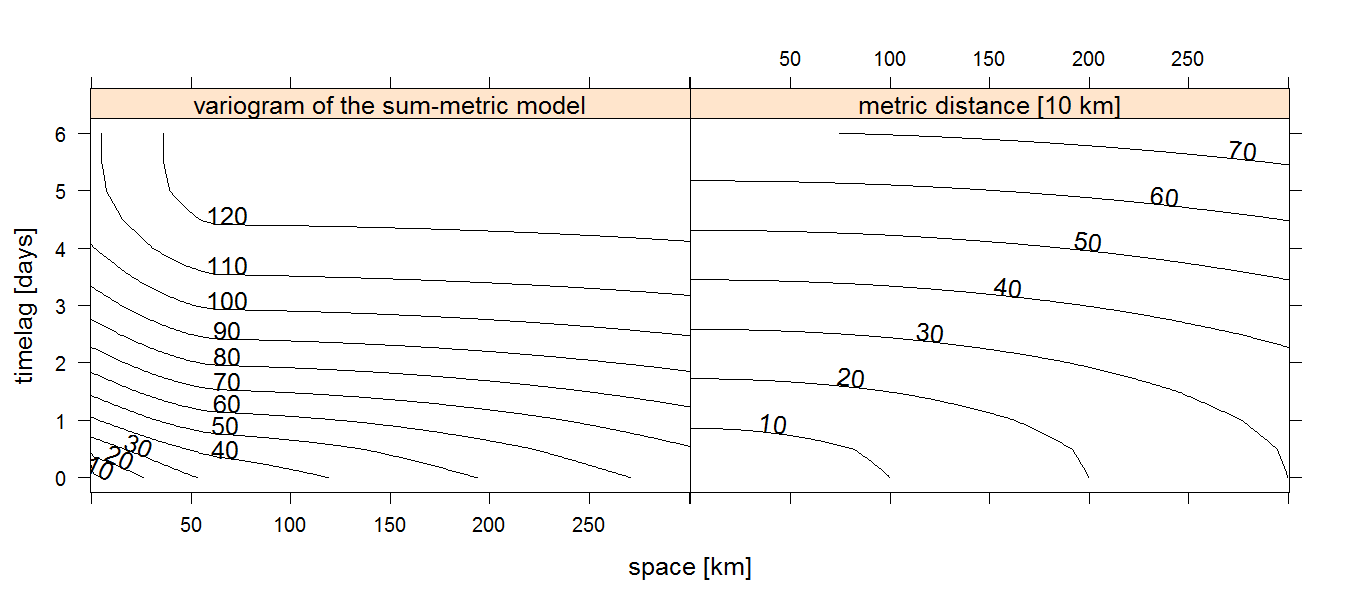
\includegraphics[width=0.9\textwidth]{vgmVsMetricDist.png}
\caption{A contourplot showing how the spatio-temporal sum-metric variogram model (as estimated in the application below) and a metric distance relate to each other. Distances are rescaled by 1/5 for easy plotting.}\label{fig:vgmVsDist}
\end{figure}

\section{Application and illustration}\label{sec:data}

The data set used is taken from AirBase\footnote{\href{http://www.eea.europa.eu/data-and-maps/data/airbase-the-european-air-quality-database-6}{AirBase - The European air quality database}}, the air quality data base for Europe provided by the European Environmental Agency (EEA). We focus on a single air quality indicator, particulate matter with a diameter less than 10~$\mu\rm m$, measured at rural background stations for 2005 (${\rm PM}_{10}$). The data base contains data for many years. Besides rural, also urban areas are monitored and not only at background locations (e.g. traffic stations). However, these processes are considered to be of a different nature and should be treated separately. As a use case, we therefore limit our data set to the rural background stations in Germany. Figure \ref{fig:dailyMeans} shows for 8 randomly chosen days daily mean values of ${\rm PM}_{10}$ concentrations for the entire monitoring network over Germany in 2005 with 69 rural background stations.

\begin{figure}
\centering
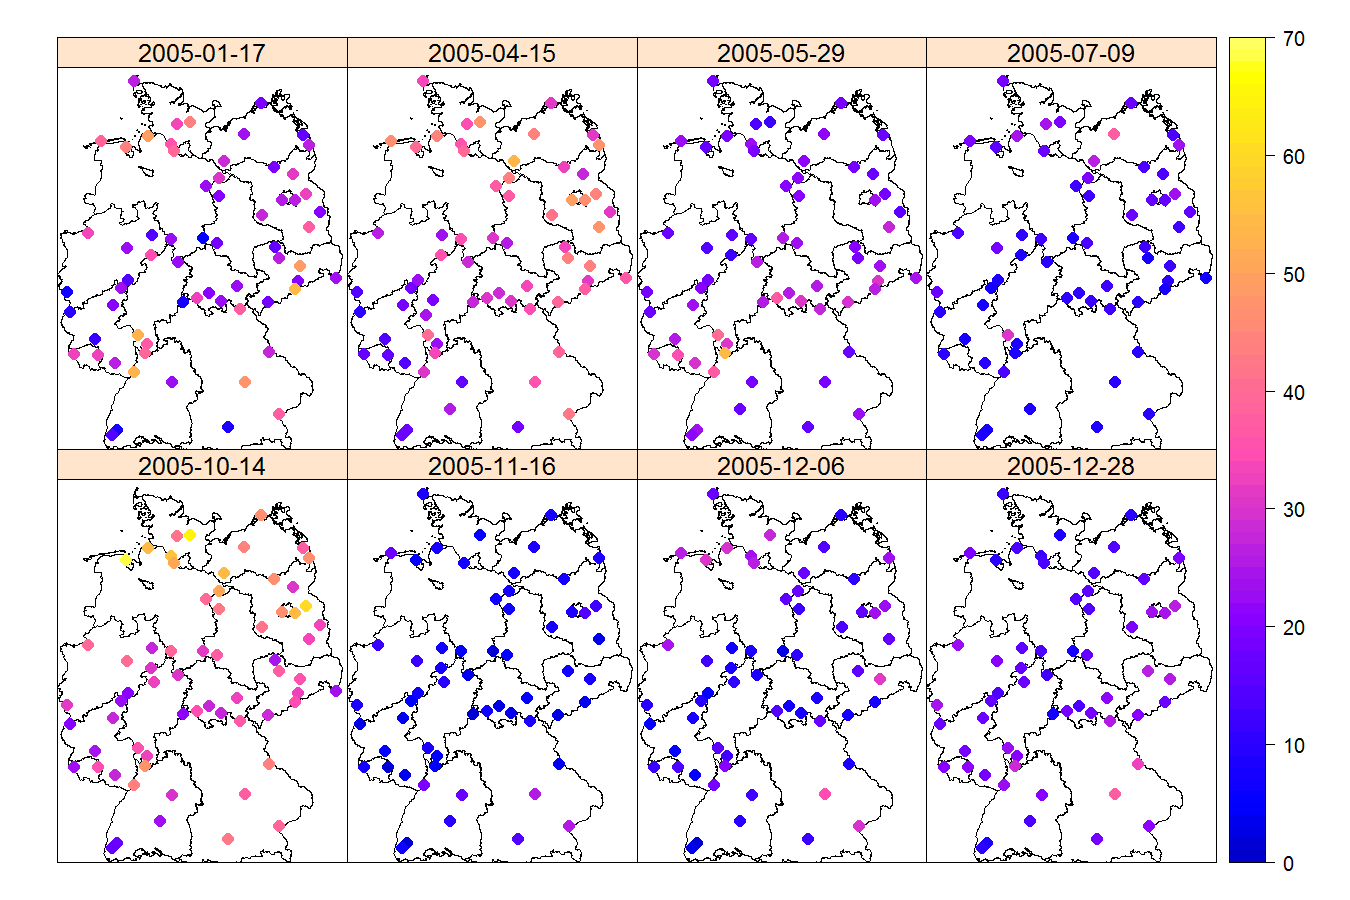
\includegraphics[width=0.95\textwidth]{daily_means_PM10.png}
\caption{Daily mean $\rm{PM}_{10}$ concentration $[\mu\rm{g/m}^3]$ at 8 randomly selected days in 2005.}\label{fig:dailyMeans}
\end{figure}

In order to fit a spatio-temporal model to the air quality data set, the empirical variogram surface is computed and used as input for the fitting routines of the different models. The empirical variogram is based on spatio-temporal bins that span regularly over space and time. 

Regular measurements over time (i.e. hourly, daily) motivate regular binning intervals of the same temporal resolution. Nevertheless, flexible binning boundaries can be passed for spatial and temporal dimensions. This allows for instance to use smaller bins at small distances and larger ones for large distances. Temporal boundaries, instead of lags, are required when the sampling of the data is non-regular. In cases where regular temporal observations can be assumed, this is utilised in the sample variogram calculations and any two temporal consecutive observations are assumed to have the same temporal distance. Figure~\ref{fig:allVgmsWireframe} shows the empirical variogram along with the proposed best fitting model of each spatio-temporal variogram family as perspective wireframe plots. In order to better identify structural shortcomings of the selected model, a difference plot (Figure~\ref{fig:allVgmsDiffWireframe}) is a helpful visual diagnostic plot.

Beyond the selection of the spatio-temporal variogram family, each component of this model can be chosen from any implemented one-dimensional variogram. In Table~\ref{tab:vgmFits} a selection of fitted models in terms of their residuals compared to the sample variogram surface are shown. The best fitting spatio-temporal model of each family is given as:

\begin{enumerate}[a)] 
\item separable model (weighted MSE: 6.82):

\nopagebreak
\begin{tabular}{l|rlrlrr}
\toprule
  & partial sill & model & \multicolumn{2}{c}{range}  & nugget & sp.-temp. sill \\ \midrule  
space & 0.86 & Exp & 558 & \hspace{-2\tabcolsep}~km & 0.14 & \multirow{2}{*}{124} \\
time & 1.00 & Sph & 5.6 & \hspace{-2\tabcolsep}~days & 0.00 & \\ \bottomrule
\end{tabular}

obtained via:

\begin{example*}
separableModel <- vgmST("separable", 
                        space = vgm(0.9, "Exp", 200, 0.1),
                        time = vgm(0.9, "Sph", 3.5, 0.1),
                        sill = 124)
fit.StVariogram(empVgm, separableModel, fit.method = 7, 
                stAni = 117.3, method = "L-BFGS-B", 
                control = list(parscale = c(100,1,10,1,100)),
                lower = c(10,0,0.1,0,0.1), 
                upper = c(2000,1,12,1,200))
\end{example*}

\item 
product-sum model (weighted MSE: 6.91)

\nopagebreak
\begin{tabular}{l|rlrlrc}
\toprule
  & partial sill & model & \multicolumn{2}{c}{range}  & nugget & k\\ \midrule  
space & 6.8 & Exp & 542 & \hspace{-2\tabcolsep}~km  & 1.2 & \multirow{2}{*}{1.61} \\
time & 8.7 & Sph & 5.5 & \hspace{-2\tabcolsep}~days & 0.0 & \\ \bottomrule
\end{tabular}

obtained via

\begin{example*}
prodSumModel <- vgmST("productSum",
                      space = vgm(10, "Exp", 200, 1),
                      time = vgm(10, "Sph",   2, 1), 
                      k=2)
fit.StVariogram(empVgm, prodSumModel, fit.method = 7, 
                stAni = 117.3, method = "L-BFGS-B", 
                control = list(parscale = c(1,10,1,1,0.1,1,10)),
                lower = rep(0.0001, 7))
\end{example*}

\item 
metric model (weighted MSE: 10.05)

\nopagebreak
\begin{tabular}{l|rlrlrrl}
\toprule
  & partial sill & model & \multicolumn{2}{c}{range}  & nugget & \multicolumn{2}{c}{anisotropy}\\ \midrule  
joint & 123.4 & ${\rm Mat}_{\kappa=0.6}$ & 453 & \hspace{-2\tabcolsep}~km & 17.4 & 189 & \hspace{-2\tabcolsep}~km/day \\ \bottomrule
\end{tabular}

obtained via

\begin{example*}
metricModel <- vgmST("metric",
                     joint = vgm(60, "Mat", 150, 10, kappa=0.6),
                     stAni = 60)
fit.StVariogram(empVgm, metricModel, fit.method = 7,
                stAni = 117.3, method = "L-BFGS-B",
                control = list(parscale = c(10,20,5,10)),
                lower = c(80,50,5,50),
                upper = c(200,1500,60,300))
\end{example*}

\item\label{bestfit} 
sum-metric model (weighted MSE: 3.31)

\nopagebreak
\begin{tabular}{l|rlrlrrl}
\toprule
          & partial sill & model & \multicolumn{2}{c}{range}  & nugget & \multicolumn{2}{c}{anisotropy}\\ \midrule  
space  & 16.4 & Sph & 67 & \hspace{-2\tabcolsep}~km    & 0 & & \\
time    &  9.3 & Exp & 0.9 & \hspace{-2\tabcolsep}~days & 0 & & \\
joint    & 91.5 & Sph & 999 & \hspace{-2\tabcolsep}~km  & 7.3 & 185 & \hspace{-2\tabcolsep}~km/day \\ \bottomrule
\end{tabular}

obtained via

\begin{example*}
sumMetricModel <- vgmST("sumMetric",
                        space = vgm(20, "Sph", 150, 1),
                        time = vgm(10, "Exp", 2, 0.5),
                        joint = vgm(80, "Sph", 1500, 2.5),
                        stAni = 120)
fit.StVariogram(empVgm, sumMetricModel, fit.method = 7, 
                stAni = 117.3, method = "L-BFGS-B", 
                control = list(parscale = c(1,100,1,1,0.5,1,1,100,1,100),
                               maxit=1e4),
                lower = c(sill.s = 0,  range.s = 10,  nugget.s = 0,
                          sill.t = 0,  range.t = 0.1,   nugget.t = 0,
                          sill.st= 0, range.st = 10, nugget.st = 0, 
                          anis = 40),
                upper = c(sill.s = 200,  range.s = 1E3,  nugget.s = 20,
                          sill.t = 200,  range.t = 75,   nugget.t = 20,
                          sill.st= 200, range.st = 5E3, nugget.st = 20,
                          anis = 500))
\end{example*}

\item 
simple sum-metric model (weighted MSE: 3.31)

\nopagebreak
\begin{tabular}{l|rlrlrlc}
\toprule
          & partial sill & model & \multicolumn{2}{c}{range} & \multicolumn{2}{c}{anisotropy} & sp.-temp. nugget \\ \midrule  
space  & 16.4 & Sph & 67   & \hspace{-2\tabcolsep}~km     & & & \multirow{3}{*}{$\Bigg\}$ 7.3} \\
time    & 9.3 & Exp & 0.9 & \hspace{-2\tabcolsep}~days & & & \\
joint    & 91.5 & Sph & 999 & \hspace{-2\tabcolsep}~km      & 185 & \hspace{-2\tabcolsep}~km/day &  \\ \bottomrule
\end{tabular}

obtained via

\begin{example*}
simpleSumMetricModel <- vgmST("simpleSumMetric",
                              space=vgm(120,"Sph", 150),
                              time =vgm(120,"Exp", 10),
                              joint=vgm(120,"Sph", 150),
                              nugget=10, stAni=150)
fit.StVariogram(empVgm, simpleSumMetricModel, fit.method = 7,
                stAni = 117.3, method = "L-BFGS-B",
                control = list(parscale = c(1,10,1,1,1,100,1,10))
                lower = c(sill.s = 0, range.s = 10,
                          sill.t = 0, range.t = 0.1,
                          sill.st= 0, range.st= 10,
                          nugget=0, anis = 40),
                upper = c(sill.s = 200,  range.s = 500,
                          sill.t = 200,  range.t = 20,
                          sill.st= 200, range.st = 5000,
                          nugget = 100, anis = 1000))
\end{example*}
\end{enumerate}

The variogram parameters are numerically optimised using the function \code{fit.StVariogram} and the \code{L-BFGS-B} routine of \code{optim}. The parameter \code{fit.method} that controls the weighing of the residuals between empirical and model surface of \code{fit.StVariogram} is set to \code{7} (the spatio-temporal analog to the commonly used spatial weighting). A full list of all weighting schemes is presented in Table~\ref{tab:weighting}. In our application, the residuals are multiplied by the number of pairs in the corresponding spatio-temporal bin divided by the metric distance: $N_j/(h_j^2 + {\rm stAni}^2\cdot u_j^2)$. The spatio-temporal anisotropy is estimated beforehand and fixed at 118~km/day. This weighting scheme puts higher confidence in lags filled with many pairs of spatio-temporal locations, but respects to some degree the need of an accurate model for short distances, as these short distances are the main source of information in the prediction step. Note, that different weighting schemes will in general result in different model parameters generating different interpolation values. Our selection is based on the assumption that well filled bins provide more reliable empirical variogram estimates and the fact that short distances are the most important ones for a local interpolation.

\begin{table}[t!]
\centering
\caption{Weighted MSE (\code{fit.method = 7, see Table~\ref{tab:weighting}}) for different spatio-temporal variogram families and different choices for the one-dimensional variogram components. Columns denote the spatial and temporal variogram choices. The metric model is only applicable if both domains use the same family.}\label{tab:vgmFits}
\begin{tabular}{ll|rrrrr}
\toprule
model & joint & Exp+Exp & Exp+Sph & Sph+Exp & Sph+Sph & ${\rm Mat}_{\kappa=0.6}$ \\ \midrule  
{separable} & $~~\cdot$ & 9.87 & \bf{6.82} & 10.42 & 7.50 & $\cdot~~$ \\
{product-sum} & $~~\cdot$ & 10.09 & \bf{6.91} & 10.64 & 7.59 & $\cdot~~$ \\
{metric} & $~~\cdot$ & 10.25 & $\cdot~~$ & $\cdot~~$ & 10.59 & \bf{10.05} \\
\multirow{2}{*}{sum-metric} & Exp &  4.10 & 3.60 & 3.89 & 3.32 & $\cdot~~$ \\
& Sph & 3.74 & 3.73 & \bf{3.31} & 3.36 & $\cdot~~$ \\
\multirow{2}{*}{simple sum-metric}& Exp &  4.10 & 3.60 & 3.94 & 3.32 & $\cdot~~$ \\
& Sph & 3.74 & 3.98 & \bf{3.31} & 3.56 & $\cdot~~$ \\ \bottomrule
\end{tabular}
\end{table}

\begin{figure}
\centering
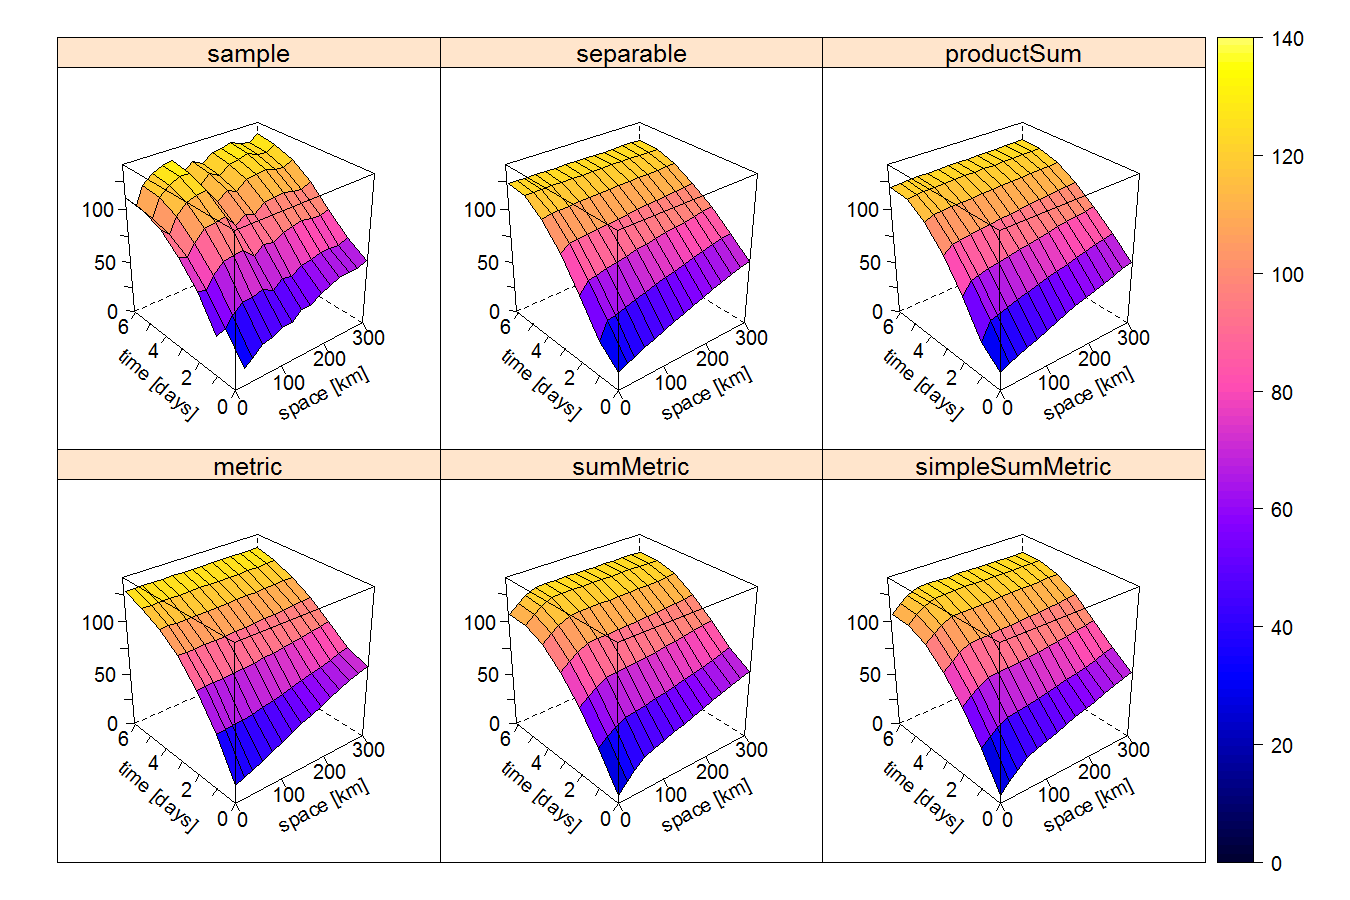
\includegraphics[width=0.95\textwidth]{allVgmsWireframe.png}
\caption{Sample and the best fitting spatio-temporal variogram of each family.}\label{fig:allVgmsWireframe}
\end{figure}

\begin{figure}
\centering
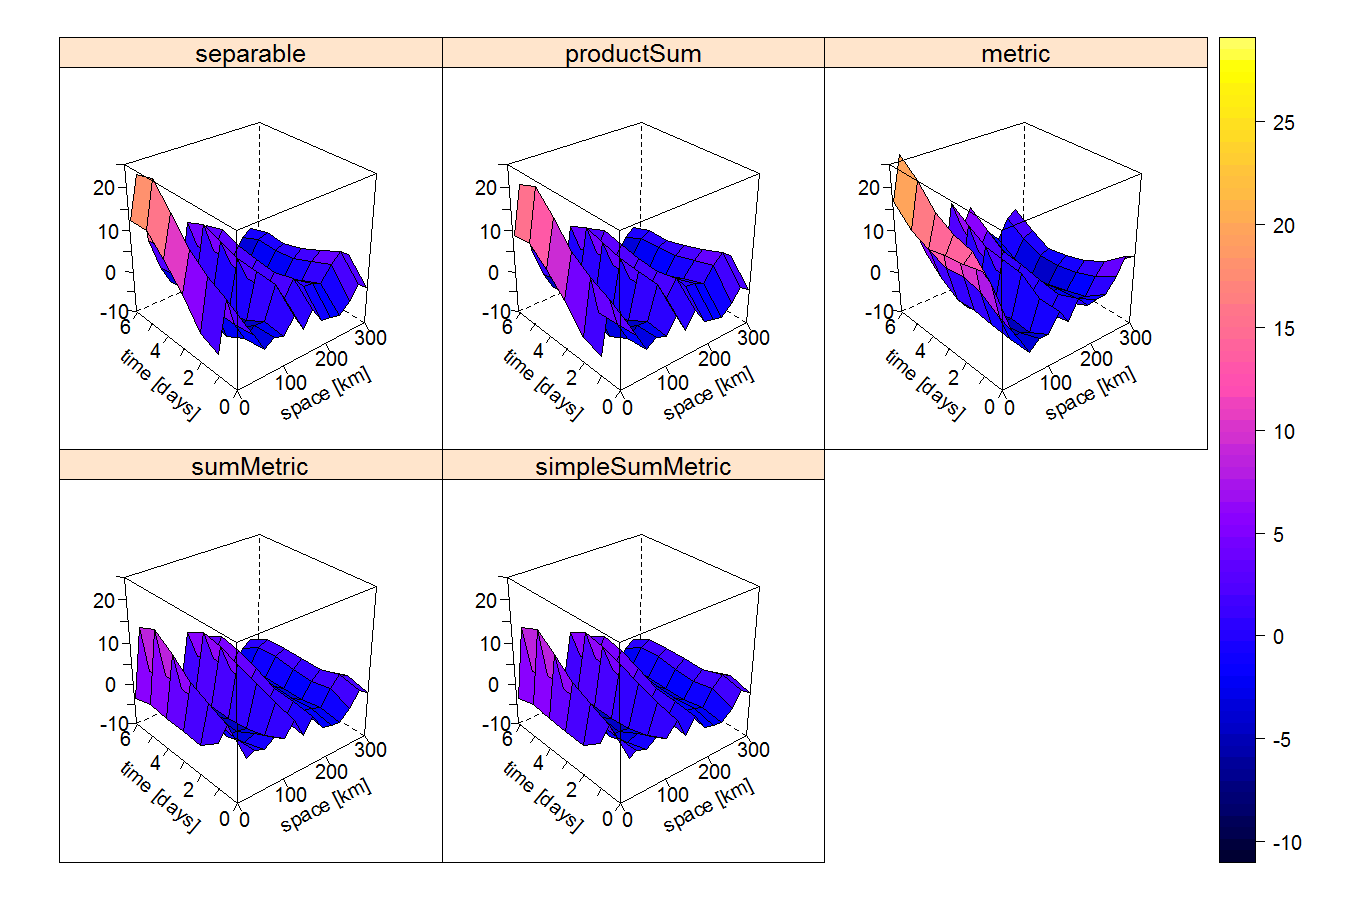
\includegraphics[width=0.95\textwidth]{allVgmsDiffWireframe.png}
\caption{Differences between the sample and the best fitting spatio-temporal variogram of each family.}\label{fig:allVgmsDiffWireframe}
\end{figure}

\begin{figure}[b!]
\centering
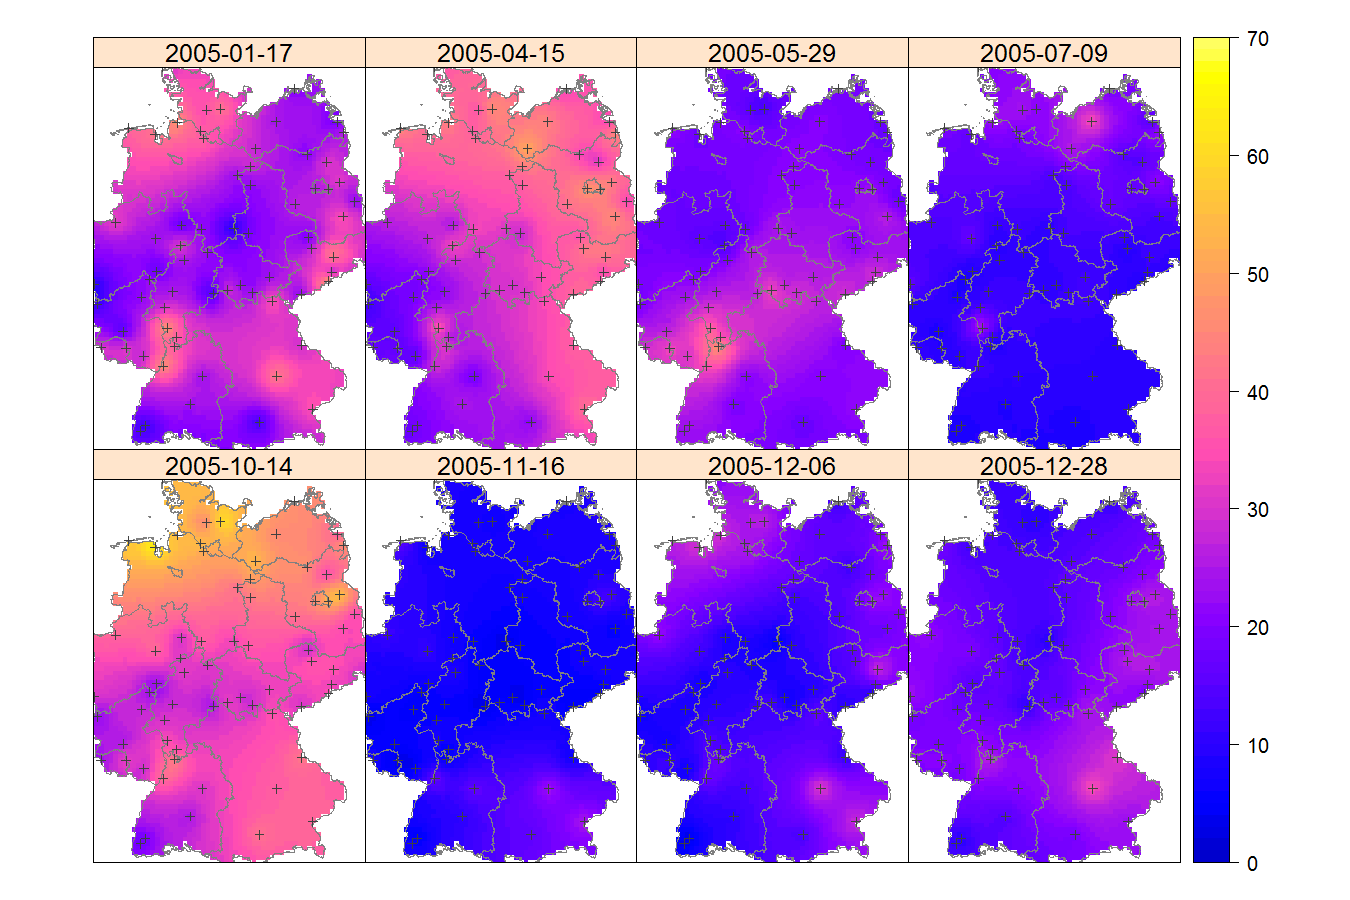
\includegraphics[width=0.95\textwidth]{pred_daily_means_PM10.png}
\caption{Spatio-temporal interpolation of daily mean $\rm{PM}_{10}$ concentrations using the sum-metric covariance model with the closest 50 neighbouring spatio-temporal locations. The crosses indicate sampling locations. The cell size of the grid in UTM projection is $10~\rm{km}\times10~\rm{km}$.}\label{fig:pred_daily}
\end{figure}

For comparison with classical approaches, we interpolate across Germany iteratively for each single day using all available data for variogram estimation. The purely spatial empirical variogram can directly be obtained from the empirical spatio-temporal variogram, by fixing the temporal lag at 0 separation. From the same set of variogram models as investigated for the spatio-temporal models, the exponential model (partial sill:~66.5, range:~224~km, nugget:~13.5) is the best suited based on the optimisation criterion. Alternatively, we could have fitted the spatial variogram for each day separately using observations from that day only. However, given the small number of observation stations, this produced unstable variograms for several days and we decided to use the single spatial variogram derived from all spatio-temporal locations treating time slices as uncorrelated copies of the spatial random field.

Once the best fitting spatio-temporal variogram model is identified, the interpolation can be executed with the help of the function \code{krigeST}. We use the sum-metric model that obtained the smallest RMSE (compare Table~\ref{tab:vgmFits}) to produce a gridded prediction. The interpolation domain consists of daily values for a regular grid spanning over Germany in UTM projection. The cell size is $10~\rm{km}\times10~\rm{km}$. Figure~\ref{fig:pred_daily} shows the interpolated grid for the same days as Figure~\ref{fig:dailyMeans} alongside with all sampling locations. Additionally, maps depicting the differences from a leave-one-out cross-validation are presented in Figure~\ref{fig:diffs_daily}. A time series view is presented in Figure~\ref{fig:timeseries} showing the observed and predicted time series at a single location along with its 95~\% prediction intervals. An animation of the entire year of daily mean ${\rm PM}_{10}$ prediction maps can be viewed online.\footnote{\url{http://gstat.r-forge.r-project.org/STpred.html}}.

The interpolated maps are generated for a set of time stamps \code{tIDs} and a grid over Germany \code{DE\_pred} by

\begin{example*}
krigeST(PM10~1, data = DE_RB_2005[ , tIDS], 
       newdata = DE_pred, fitSumMetricModel, nmax = 50,
       stAni = fitMetricModel$stAni/24/3600)
\end{example*}

\begin{figure}[t!]
\centering
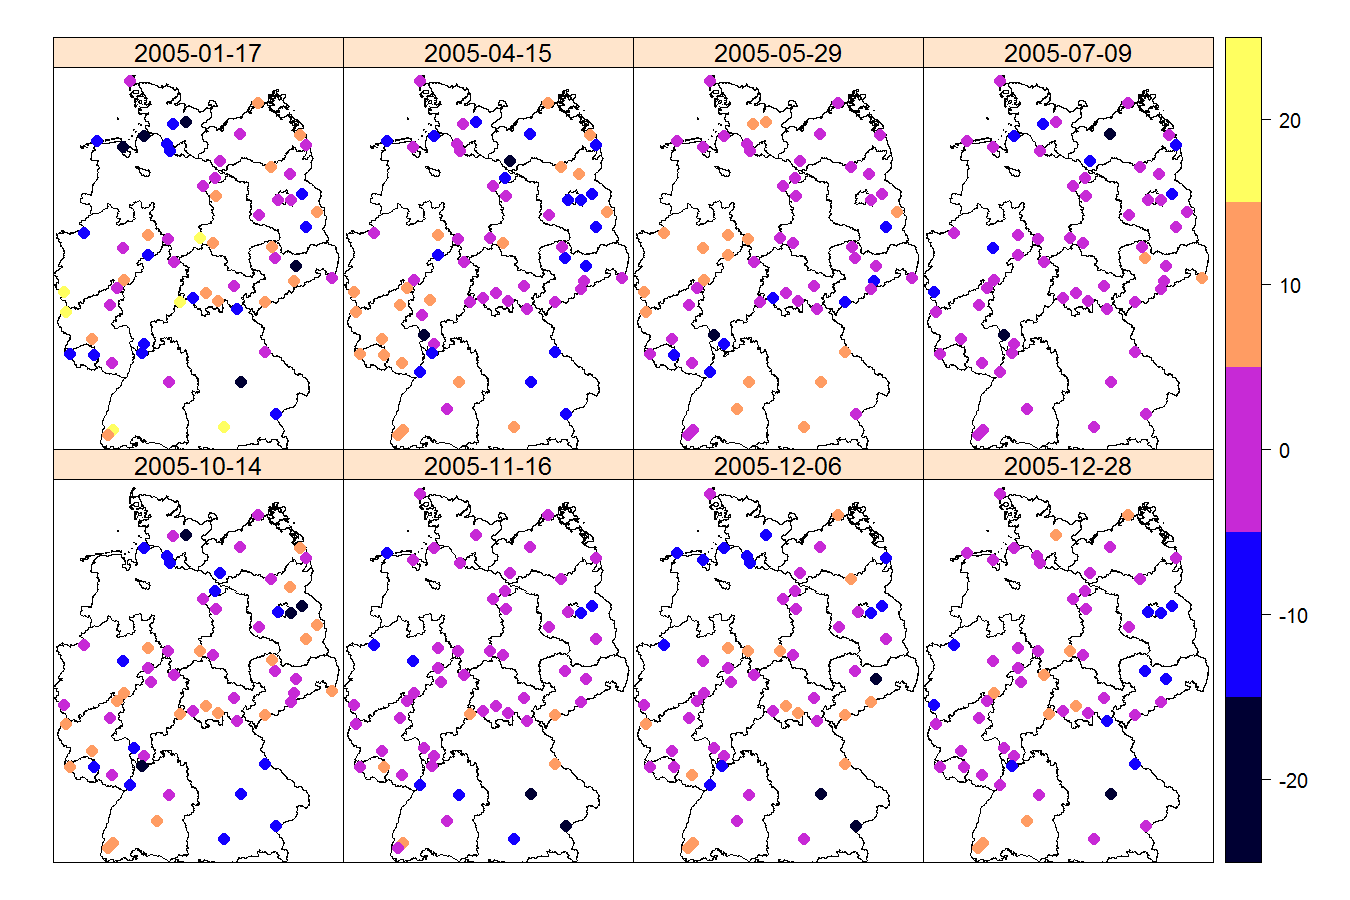
\includegraphics[width=0.95\textwidth]{diffs_daily_means_PM10.png}
\caption{Differences of spatio-temporal predictions and observed daily mean $\rm{PM}_{10}$ concentrations using the sum-metric covariance model with the closest (approx. strongest correlated) 50 neighbouring spatio-temporal locations.}\label{fig:diffs_daily}
\end{figure}

\begin{figure}[h!]
\centering
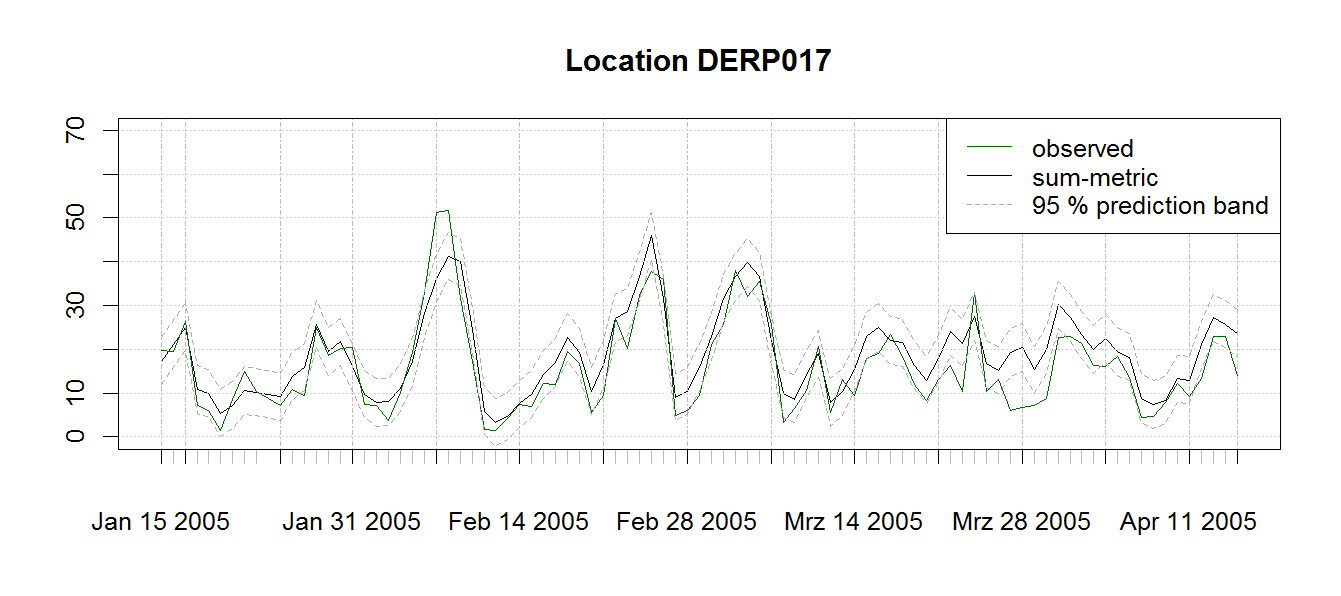
\includegraphics[width=0.9\textwidth]{singleStationTimeSeries.png}
\caption{Subset of the time series of observed and predicted ${\rm PM}_{10}$ at a single station in Lower Saxony along with its 95~\% prediction intervals.}\label{fig:timeseries}
\end{figure}

To further compare the different approaches, a leave-one-out cross-validation was carried out. The spatio-temporal interpolations are done for the closest 50 and 10 neighbours assessing the impact of the neighbourhood size. Inspection of the ranges of the variograms in the temporal domain, suggests that any station more than at most 6 days apart does not meaningfully contribute. Furthermore, the local estimation allows the spatio-temporal random field to have a varying mean value over space and time. The purely spatial interpolation can be considered as the extreme temporally local case, where only observations from the same time instance are considered.


\begin{table}
\caption{Leave-one-out cross-validation results. The column wMSE refers to the optimised value from the variogram estimation.}\label{tab:cv}
\centering
\begin{tabular}{lrr|rrrr}
\toprule
covariance model & wMSE & neigh. &  RMSE   &   MAE   &    ME   &   COR \\ \midrule
pure Spatial & & 10 & 6.15 & 4.09 & -0.01 & 0.84 \\
separable &\hspace{-\tabcolsep}[6.82]&     10 & 6.08 & 4.04 & -0.01 & 0.84  \\
product-sum &\hspace{-\tabcolsep}[6.91]& 10 &  6.08& 4.04& -0.01 & 0.84  \\ 
metric &\hspace{-\tabcolsep}[10.05]&          10 &  6.11 & 4.07 & 0.03 & 0.84  \\ 
sum-metric &\hspace{-\tabcolsep}[3.31]&   10 &  6.16 & 4.08 & -0.06 & 0.84  \\ 
simple sum-metric &\hspace{-\tabcolsep}[3.31]& 10 & 6.14 & 4.08 & -0.02 & 0.84  \\  \midrule
pure Spatial & & 50 & 6.10 & 4.07 & 0.00 & 0.84  \\
separable &\hspace{-\tabcolsep}[6.82]& 50     &  6.05 & 4.04 & 0.01 & 0.84  \\ 
product-sum &\hspace{-\tabcolsep}[6.91]& 50 &  6.05 & 4.04 & 0.00 & 0.84  \\ 
metric &\hspace{-\tabcolsep}[10.05]& 50          &  6.07 & 4.08 & 0.03 & 0.84  \\ 
sum-metric &\hspace{-\tabcolsep}[3.31]& 50   &  6.14 & 4.09 & -0.01 & 0.84  \\ 
simple sum-metric &\hspace{-\tabcolsep}[3.31]& 50 &  6.14 & 4.08 & -0.02 & 0.84 \\ \bottomrule
\end{tabular}
\end{table}

\section{Results and discussion}\label{sec:resultsDiscuss}

In terms of added value of spatio-temporal kriging measured in cross-validation results, Table~\ref{tab:cv} shows hardly any benefit in the illustrative example. This effect can to a large degree already be explained from the spatio-temporal variograms: a temporal lag of one or a few days leads already to a large variability compared to spatial distances of few hundred kilometres, implying that the temporal correlation is too weak to considerably improve the overall prediction. Nevertheless, investigating a process with a higher temporal frequency will likely show a stronger correlation in the temporal domain. Looking into station-wise cross-validation statistics (not shown), the four stations with an RMSE of 10 and larger correspond to the locations with the largest annual mean concentrations ($>22~\mu{\rm g}/{\rm m}^3$).
 
The added value of spatio-temporal kriging lies in the flexibility of the model. We are now in the position to not only interpolate at unobserved locations in space, but also at unobserved time instances. This makes spatio-temporal kriging a suitable tool to fill gaps in time series not only based on the time series solely, but also including some of its spatial neighbours. A very irregular sampled data set would as well largely benefit from a spatio-temporal approach, as spatially close but unobserved locations in one time slice are not of any help in a purely spatial approach, but the spatio-temporal model would benefit from the observed value nearby at another time instance. In a completely regular data set, the distance to a spatio-temporal neighbour is at least as large as the pure spatial distance and hence the correlation is weaker. Furthermore, being able to capture the covariance structure over space and time might foster a better understanding of the process under study. 

While we see spatio-temporal modelling being a powerful tool, the cross-validation results in Table~\ref{tab:cv} show that spatio-temporal kriging will not solve the problem of all poorly spatially captured phenomena. Further preprocessing steps might be necessary to improve the modelling of this $\rm{PM}_{10}$ data set such as for instance a temporal AR-model followed by spatio-temporal residual kriging or using further covariates in a preceding (linear) modelling step. Providing the best possible model of $\rm{PM}_{10}$ concentrations across Germany was beyond the scope of this paper.

The selection of a spatio-temporal covariance model should not only be made based on the (weighted) mean squared difference between the empirical and model variogram surfaces (presented in Table~\ref{tab:vgmFits}), but also on conceptional choices and visual (Figure~\ref{fig:allVgmsWireframe}) judgement of the fits. Even though the function \code{fit.StVariogram} provides optimisation routines to fit different spatio-temporal variogram models, the numerical routines in the background may struggle to find the optimal parameters. Besides the lower and upper boundaries of the parameter space, the control parameter \code{parscale} of the \code{optim} function is  a valuable option to improve the convergence of the optimisation. With passing \code{parscale} as entry of the list \code{control} a vector of scalars must be passed that controls the different levels of magnitude of the variogram parameters. In most applications, a change of 1 in the sills will have a stronger influence on the variogram surface than a change of 1 in the ranges. The problem becomes more difficult with an increasing number of parameters. In our application, using the simple sum-metric model as starting values for the full sum-metric model improved the convergence speed of the more complex model. In the presented application, the sum-metric models turns out to be the same as the simple sum-metric model. While this might at first sight be due to using the simpler model to generate starting values, different non simplified starting models converged to the same result. 

Generally, it is important to keep in mind the strong interaction of the model parameters. It is typically not easy to distinguish how much of the spatio-temporal nugget and sill is attributed to spatial, temporal or joint components. In this paper we considered a joint numerical approach, but step-wise approaches where the components are estimated separately could as well be considered. The interested reader is also referred to \cite{Nash2014}. However, all optimisation approaches follow the premise that the studied process can be approximated with the given model and available data. If this premise fails, no optimal model can be selected.

An extension towards a restricted maximum likelihood method (REML) to fit the spatio-temporal variogram model would be desirable, as it overcomes some of the above mentioned drawbacks of the method of moments based approaches and would additionally provide standard errors for the parameter estimates. A REML approach would allow to take into account that sample variogram values are correlated. However, for large datasets (as in the spatio-temporal case), it is computationally more feasible to use a least squares fitting. To reduce the correlation of the variogram values, some randomisation could be implemented in large data sets, to calculate the sample variogram based on partially overlapping or even disjoint sets of observations.

The selected anisotropy as proxy to the relation of spatial and temporal distance in determining the strongest correlated neighbours might show a distortion for some models when only few neighbours are used towards the true set of the most correlated locations. However, this effect vanishes as soon as the spatio-temporal range of the model is sufficiently represented through the set of nearest neighbours. 

As mentioned by \cite{kj99}, an alternative to space-time kriging might be co-kriging. However, this is only feasible if the number of time replicates is (very) small, as the number of cross variograms to be modelled equals the number of {\em pairs} of time replicates. Also, co-kriging can only interpolate for these time slices, and not inbetween or beyond them. It does however provide prediction error covariances, which can help assessing the significance of estimated {\em change} parameters \citep{pe1,pe2}. Several of the space-time variograms presented here may be approximated by sets of direct variograms and cross-variograms.

Fitting variogram models to sample space-time variograms is in our implementation done by \code{stats::optim}.  Our example script uses method \code{L-BFGS-B} and provides upper and lower parameter boundaries, e.g. to make sure sill parameters do not become negative. There has been a lot of research in optimization since the methods in \code{optim}, some of which has been reported in the special issue of the Journal of Statistical Software \citep{optim}, and we do see potential to improve the options in this respect.

The approximate selection of the most correlated neighbours solves the lack of a natural notion of a joint distance across space and time. However, other sampling properties might introduce a bias in the prediction. The prediction at an unobserved location with a cluster of observations at one side will be biased towards this cluster and neglect the locations towards the other directions. Similar as the quadrant search in the pure spatial case an octant wise search strategy for the local neighbourhood would solve this limitation. A simpler stepwise approach to define an $n$-dimensional neighbourhood might already be sufficient in which at first $n_s$ spatial neighbours and then from each spatial neighbour $n_t$ time instances are selected, such that $n_s \cdot n_t \approx n$.

The presented example considers stationary random fields that are isotropic in space. Further extensions towards more sophisticated variogram estimations allowing also for spatial geometric anisotropy are desirable. One could for instance plot variogram maps for spatial separation in North and South direction for each temporal lag. However, the current implementation does not allow to use the anisotropy parameter \code{anis} of the pure spatial variogram definition. Nevertheless, a preliminary rescaling of coordinates would be a possible workaround. This route has for instance been taken by \citet{Gasch2015} performing 3D+T kriging . The soil profiles in their study show a clear difference in horizontal and vertical variography. To correct for this, the depth dimension of the data has been rescaled to correspond with the dimensions of the horizontal distances before hand. In the subsequent study, these pseudo 3D coordinates have been used to fit the spatio-temporal variograms and perform kriging. 

The code in model definitions is meant to be kept both flexible and simple. This is based on i) re-producing the notion of the geostatistical models in the R code and in ii) reusing existing definitions and functions of the pure spatial cases that have been available for many years in \pkg{gstat}. The data handling benefits to a large degree from the implementations in the \pkg{spacetime} R package.


\section{Conclusions}\label{sec:conclusions}

The spatio-temporal extensions to \pkg{gstat} allow to model a set of spatio-temporal covariance functions. The implemented functionality eases estimation, visualisation and understanding of spatio-temporal covariance functions. The extension and reuse of already available function structures and nomenclature facilitates an easy translation of spatial workflows to handle spatio-temporal data. The numerical estimation of the variogram parameters might be tricky and needs a large degree of the users attention. It is advised to carefully check the outcome of the \code{optim} routine after optimisation. Spatio-temporal kriging predictions can be made in a global and a local neighbourhood set-up, while the latter will be the preferred solution for most spatio-temporal data sets and common computer hardware configurations. 

Spatio-temporal covariance structures carry valuable information, but a spatio-temporal model is not guaranteed to outperform pure spatial predictions. The benefit in terms of prediction quality of spatio-temporal kriging becomes only apparent if sufficiently strong correlated locations are added with the temporal dimension (i.e., if the model permits strong correlation across time). Nevertheless, the spatio-temporal covariance model might be of interest in itself. 

Besides some publications where the authors of this paper were involved in, such as \cite{Kilibarda2014}, the software presented here has proven useful in several independent publications, examples of which are \citep{marek, biondi, hu, yoon}.

\section*{Acknowledgements}
This research has partly been funded by the German Research Foundation (DFG) under project number PE 1632/4-1. We thank two anonymous reviewers for their valuable comments.

\bibliography{spatio-temporal-kriging}

\pagebreak

\address{Benedikt Gr{\"a}ler\\
  Institute for Geoinformatics, University of M{\"u}nster\\
  Heisenbergstr. 2, 48149 M{\"u}nster\\
  Germany}\\
\email{ben.graeler@uni-muenster.de}

\address{Edzer Pebesma\\
  Institute for Geoinformatics, University of M{\"u}nster\\
  Heisenbergstr. 2, 48149 M{\"u}nster\\
  Germany}\\
\email{edzer.pebesma@uni-muenster.de}

\address{Gerard Heuvelink\\
  Department of Environmental Sciences, Wageningen University\\
  street, code, city\\
  The Netherlands}\\
\email{gerard.heuvelink@wur.nl}

\section*{Appendix}
\subsection*{Derivation of the separable covariance and variogram identities}\label{sec:derivSep}

The separable covariance and variogram identity is readily available through

\begin{eqnarray*}
C_{\rm sep}(h,u) &=& C_{\rm s}(h)C_{\rm t}(u) = sill \cdot \bar{c}_s(h)\bar{c}_t(u) \\
\gamma_{\rm sep}(h,u) &=& C_{\rm sep}(0,0) - C_{\rm sep}(h,u) \\
 &=& sill \big(1- \bar{c}_s(h) \cdot \bar{c}_t(u) \big) \\
 &=& sill \big(1- \big(1-\bar{\gamma}_s(h)\big)\big(1-\bar{\gamma}_t(u)\big) \big) \\
 &=& sill \big(1- \big(1-\bar{\gamma}_s(h) -\bar{\gamma}_t(u) + \bar{\gamma}_s(h)\bar{\gamma}_t(u)\big) \big) \\
 &=& sill \big(\bar{\gamma}_s(h) + \bar{\gamma}_t(u) - \bar{\gamma}_s(h)\bar{\gamma}_t(u)\big)
\end{eqnarray*}

where $\bar{c}$ and $\bar{\gamma}$ are normalised correlation and correlogram functions respectively.

\subsection*{Derivation of the product-sum covariance and variogram identities}\label{sec:derivPs}

The product-sum covariance and variogram identity is readily available through:
\begin{eqnarray*}
C_{\rm ps}(h,u) &=& k \cdot C_{\rm s}(h)C_{\rm t}(u) + C_{\rm s}(h) + C_{\rm t}(u) \\
\gamma_{\rm ps}(h,u) &=& C_{\rm ps}(0,0) - C_{\rm ps}(h,u) \\
 &=& k \cdot C_{\rm s}(0)C_{\rm t}(0) + C_{\rm s}(0) + C_{\rm t}(0) \\
 &  & - \big(k \cdot C_{\rm s}(h)C_{\rm t}(u) + C_{\rm s}(h) + C_{\rm t}(u)\big) \\
 &=& k \cdot {\rm sill}_{\rm s} \cdot {\rm sill}_{\rm t} + {\rm sill}_{\rm s} + {\rm sill}_{\rm t} \\
 &  & - k \cdot \big[ \big({\rm sill}_{\rm s} - \gamma_{\rm s}(h)\big)\big({\rm sill}_{\rm t} - \gamma_{\rm t}(u)\big)\big] - \big({\rm sill}_{\rm s} - \gamma_{\rm s}(h)\big) - \big({\rm sill}_{\rm t} - \gamma_{\rm t}(u)\big) \\
 &=&  k \cdot {\rm sill}_{\rm s} \cdot {\rm sill}_{\rm t} + {\rm sill}_{\rm s} + {\rm sill}_{\rm t} \\
 &   & - k \cdot \big[ {\rm sill}_{\rm s} \cdot {\rm sill}_{\rm t} - {\rm sill}_{\rm s} \cdot \gamma_{\rm t}(u) - {\rm sill}_{\rm t} \cdot \gamma_{\rm s}(h) + \gamma_{\rm s}(h) \gamma_{\rm t}(u) \big] \\
 & & - {\rm sill}_{\rm s} + \gamma_{\rm s}(h) - {\rm sill}_{\rm t} + \gamma_{\rm t}(u) \\
 &=& k \cdot {\rm sill}_{\rm t} \gamma_{\rm s}(h) + k \cdot {\rm sill}_{\rm s} \gamma_{\rm t}(u) - k \gamma_{\rm s}(h) \gamma_{\rm t}(u) + \gamma_{\rm s}(h) + \gamma_{\rm t}(u) \\
 &=& (k \cdot {\rm sill}_{\rm t} + 1) \gamma_{\rm s}(h) + (k \cdot {\rm sill}_{\rm s} + 1) \gamma_{\rm t}(u) - k \gamma_{\rm s}(h) \gamma_{\rm t}(u)
\end{eqnarray*}
